\newpage
\mychapter{Основные уравнения}
В данной работе использовано несколько уравнений. Эти уравнения
достаточно широко известны, поэтому здесь им уделено всего несколько
слов.

Гамильтониан NV-центра:
\begin{equation}\label{eq:shamiltonian}
\hat{H} = \hbar\cdot D\cdot \hat{S_z^2} + \hbar\cdot E\cdot (\hat{S_x^2} - \hat{S_y^2}) +
g_e\cdot \mu_B\cdot (\hat{\vec{S}}, \vec{B})
\end{equation}
Здесь $D$=$2.877$ ГГц и $E$=$7.7$ МГц --- продольная и поперечная
компоненты тензора энергии расщепления в кристаллическом поле
электронных спиновых состояний, $g_e$=$2.0028$ --- электронный фактор
Ланде, $\mu_B$=$5.788 \cdot 10^{-9}$эВ/Гс --- магнетон Бора,
$\hbar$=$4.135 \cdot 10^{-15}$ эВ $\cdot$ с --- постоянная Планка. 
Спектр NV-центра показан на рисунке (\ref{fig:nv-spectrum}). 
\begin{figure}[H]\centering
  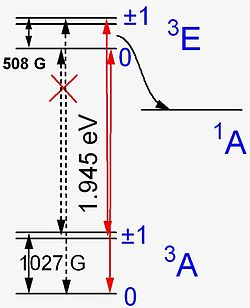
\includegraphics[width=0.5\textwidth]{nv-spectrum}
  \caption{Спектр NV-центра в алмазе.}\label{fig:nv-spectrum}
\end{figure}

Все
расчеты в работе произведены в базисе спиновых состояний NV-центра:
\[ 
   |m_s=+1> = \left(
   \begin{array}{c}
   1 \\ 0 \\ 0
   \end{array} \right),
   |m_s=0> = \left(
   \begin{array}{c}
   0 \\ 1 \\ 0
   \end{array} \right),
   |m_s=-1> = \left(
   \begin{array}{c}
   0 \\ 0 \\ 1
   \end{array} \right)
\]
в этом базисе спиновые операторы выглядят так:
\[
   S_x = \frac{1}{\sqrt{2}} \left(
   \begin{array}{ccc}
    0 & 1 & 0 \\
    1 & 0 & 1 \\
    0 & 1 & 0
   \end{array} \right),
   S_y = \frac{1}{i \sqrt{2}} \left(
   \begin{array}{ccc}
    0 & 1 & 0 \\
    -1 & 0 & 1 \\
    0 & -1 & 0
   \end{array} \right),
   S_z = \frac{1}{\sqrt{2}} \left(
   \begin{array}{ccc}
    1 & 0 & 0 \\
    0 & 0 & 0 \\
    0 & 0 & -1
   \end{array} \right).
\]

Частота Раби:
\[ 
\Omega_R = g_e \cdot \mu_B \cdot B
\]
количественно описывает взаимодействие резонансного магнитного поля со
спином NV-центра. Под действием резонансного излучения амплитудой $B$
заселенность уровней осциллирует с частотой Раби.
